\documentclass[12pt,parskip]{komatufte}
\usepackage[subpreambles=false]{standalone}

%%%%%%%%%%%%%%%%%%%%%%%%%%%
% Silence warning messages
\usepackage{silence}
\WarningsOff[scrlayer-notecolumn]
\WarningsOff[biblatex]

%%%%%%%%%%%%%%%%%%%%
% Commenting

%\usepackage[author=Lyndon]{pdfcomment}
%\newcommand{\pdfcomment}[1]{} %ignore all comments

%\usepackage{todonotes}
%\newcommand{\pdfcomment}{\todo}


%%%%%%%%%%%%%%%%%%%%
% Tables
\usepackage{booktabs}

%%%%%%%%%%%%%%%%%%%
% Fonts
\usepackage{tgadventor} %sans
\usepackage{tgpagella}  %serif
\usepackage{inconsolata} %mono
\usepackage[T1]{fontenc}

\usepackage{microtype}
\usepackage[all]{nowidow}
%%%%%%%%%%%%%%%%%%%%%%%
% Styling
\setcounter{secnumdepth}{4}
\setcounter{tocdepth}{2}

\usepackage{placeins}



%%%%%%%%%%%%%%%%%%%
% Math
\usepackage{amsmath, amssymb, stmaryrd, mathtools}
\DeclareMathOperator*{\argmin}{argmin}
\DeclareMathOperator*{\argmax}{argmax}

\usepackage{xparse,xstring,etoolbox}
% crossref this against notation section
\newcommand{\vv}[1]{\tilde{#1}} % vector
\newcommand{\seq}[1]{\mathcal{#1}} % sequence
\newcommand{\set}[1]{\mathbb{#1}} % set

%%%%%%%%%
% Indexing/sequence indexing
\newcommand{\seqind}[2]{#1^{#2}} % seqence index
\newcommand{\ind}[2]{#1_{#2}} % indexed
\newcommand{\disamb}[2]{#1^{\mathrm{#2}}} %disambiguated

%% Smart indexing and naming
\newcommand{\ifupper}[3]{
    \normalexpandarg
	\exploregroups
	\StrCount{ABCDEFGHIJKLMNOPQRSTUVWXYZ}{#1}[\uppercount]
	\ifnumgreater{\uppercount}{0}{#2}{#3}
}

%smart index
\DeclareDocumentCommand{\ii}{u{_} m}{
	\ifupper{#1}%
	{% just a single uppercase character, i.e. a matrix
		  %make sure the index is the right length
		\StrCount{#2}{,}[\indcount]
		\ifnumgreater{\indcount}{0}
		{ % Got multiple indexes so all good
		 	\ind{#1}{#2}
		}
		{ % Only 1 index so grab the column
		 	\ind{#1}{{:,#2}}
		}
	}%
	{% Not just a single upper case character
		\ind{#1}{#2}
	}
}

\DeclareDocumentCommand{\nn}{u{_} m}{
	\seqind{#1}{#2}
}

\DeclareDocumentCommand{\dd}{u{_} m}{
	\disamb{#1}{#2}
}

% Index of a vector
\DeclareDocumentCommand{\iv}{u{_} m}{\ii{\vv #1}_{#2}}
\DeclareDocumentCommand{\dv}{u{_} m}{\dd{\vv #1}_{#2}}
\DeclareDocumentCommand{\nv}{u{_} m}{\nn{\vv #1}_{#2}}

%exp
\let\oldexp\exp
\renewcommand{\exp}[1]{\oldexp \left( #1 \right)}
\newcommand{\exptwo}[1]{\oldexp_2 \left( #1 \right)}

\newcommand{\softmax}{\mathrm{smax}}

\DeclareMathOperator*{\expectedop}{\mathbb{E}}
\DeclareDocumentCommand{\expected}{u{_} m}{
	\expectedop\limits_{\mathrlap{#2}}
}

%%%%%%%%%%%%%%%%
%Graphics
\usepackage{tikz}
\usetikzlibrary{positioning, fit,  shapes.geometric}
\usepackage{ifthen}
\usepackage{etoolbox}

\tikzset{
	backgroundcolor/.style ={fill=white},
	every node/.append style={
		minimum height=7mm,
	},
	labe/.append style={
		%Blue,
		align = center,
		backgroundcolor,
		fill opacity=0.6,
		text opacity=1,
		font={\footnotesize\itshape}	
	},
	layer/.append style={
		draw,
		align = center,
		minimum height=7mm,
	},
	tight/.append style={
		inner sep=0.2mm,
	},
	lookupbox/.append style={
		draw=none,
		append after command={
		       	[shorten <= -0.5\pgflinewidth]
		       	([shift={(-1.5\pgflinewidth,-0.5\pgflinewidth)}]\tikzlastnode.north east)
		       	edge([shift={( 0.5\pgflinewidth,-0.5\pgflinewidth)}]\tikzlastnode.north west) 
		       	([shift={( 0.5\pgflinewidth,-0.5\pgflinewidth)}]\tikzlastnode.north west)
		       	edge([shift={( 0.5\pgflinewidth,-1.5\pgflinewidth)}]\tikzlastnode.south west)            
		       	([shift={( -1.5\pgflinewidth,+0.5\pgflinewidth)}]\tikzlastnode.south east)
		       	edge([shift={(-1.5\pgflinewidth,-0.5\pgflinewidth)}]\tikzlastnode.north east)
		},
		inner sep=0.7mm,
		outer sep=0mm,
		minimum width=25mm
	}
}

\usepackage{pgfplots}
\pgfplotsset{compat=1.14}
\pgfplotsset{sideplot/.append style={
		width=\notescolwidth,
		domain=-10:10,
		samples=101,
		smooth,
		enlarge y limits={abs=2},
		axis lines=middle,
		xlabel  = $z$,
		ylabel  = $y$,
	},
	equ/.append style={
		color=blue,
		thick,
		mark=none
	}
}

% Function  For a plot 
% it  needs to be declared in preamble because of how \makenote* interacts with multiple files
\def\errorsurface(#1,#2){(0.5*#1 + 0.7*#2 + sin(deg(1.5*#1 + #2^2)))^2}


\usepackage{graphicx}
\graphicspath{{./figs/}, {./}, {./figs/chaptersentencerrepr/}, {./figs/chapterintromachinelearning/}, {./figs/chapterwordrepr/}}
\usepackage{adjustbox}


%%%%%%%%%%%%%%%%%%%
% Refs
\usepackage{cleveref}

\addbibresource{master.bib}

%%%%%%%%%%%%%%%%%%%%
% Formatting

% for examples from natural language space.
\newcommand{\natlang}[1]{\ifmmode \text{``\texttt{#1}''} \else {``\texttt{#1}''}\fi}
% \ifmmode ``trick'' from https://tex.stackexchange.com/a/15194/5834

%%%%%%%%%%%%%%%%%%%%%



\begin{document}

\setchapterpreamble{%
	\dictum[\textit{English Composition and Literature}, Webster, 1923]
	{
		A sentence is a group of words expressing a complete thought.
	}
}
\chapter{Sentence Representations and Beyond}\label{sec:sentence-representations-and-beyond}
\begin{abstract}
	This chapter discusses representations for larger structures in natural language.
	The primary focus is on the sentence level.
	However, many of the techniques also apply for sub-sentence structures (phrases), and super-sentence structures (documents).
	The three main types of representations discussed here are: unordered models, such as sum of word embeddings; sequential models, such as recurrent neural networks; and structured models, such as recursive autoencoders.
\end{abstract}


\aside[Word Sense Embeddings as a by-product]{
	Almost all sentence representation methods product word embeddings as a by-product
	Either output embeddings, from the softmax,
	or input embeddings that are used as the networks inputs.}
\aside[Initialising input embeddings]{
	In the case of systems with input embeddings it is common (but not ubiquitous) to initialise them using a pretrained embeddings from one of the methods discussed in the \Cref{sec:word-representations},
	then allow them to be fine-tuned while training the sentence embeddings.
}


It can be argued that the core of true AI,
is the capture and manipulate the representation of an idea.
In natural language a sentence (as defined by Webster in the quote above),
is such a representation of an idea, but it is not machine manipulatable.
As such the conversion of sentences to a machine manipulatable representation is an important task in AI research.


All techniques which can represent documents (or paragraphs) can by necessity represent sentences as well.
A single sentence can be a whole document, similarly for paragraphs.
Many of these models always work for sub-sentence structures also, like key-phrases.
The reverse is not necessarily true: most documents are not just a single sentence.
When considering on documents beyond sentences,
neural network embedding models directly compete with vector information retrieval models.
These include LSI \pcite{dumais1988using}, probabilistic LSI \pcite{hofmann2000learning} and  LDA \pcite{blei2003latent}.

\pdfcomment{I need to get my head straight about when these models are like word embeddings vs when they are like document embeddings. I think it is just taking on output instread of the other, but it has been a while since I looked at this}

\aside[Word Sense Embeddings in Sentence Embeddings]{
While the last chapter was all about sense embeddings, they are unmentioned here.
One might think that they would be very useful for sentence embeddings.
However, they are not as needful as one might expect.
The sense of a word being used is determined by the context.
Ideally, it is determined by what the context means.
As a sentence embedding is a direct attempt to represent the meaning of such a context, determining the sense of each word within is not a requirement.
Using sense embeddings instead of word embeddings is a valid extension to many of these methods.
However it requires performing word sense disambiguation.
Which as discussed in the previous chapter is very difficult.
}



\section{Unordered and Weakly Ordered Representations}

A model that does not take into account word order can not perfectly capture the meaning of an a sentence.
\tcite{Mitchell2008} give the poignant examples of:
\begin{itemize}
	\item \natlang{It  was  not  the  sales  manager who  hit  the  bottle that day, but the office worker with the serious drinking problem.}
	\item \natlang{That  day  the  office  manager,   who  was drinking, hit the problem sales worker with a bottle, but it was not serious.}
\end{itemize}
These two sentences have the same words, but in a different structure, given them a very different meanings.
However, in practice representations which discard word order can be quiet effective.


\subsection{Sums of Word Embeddings}
\aside[SOWE is a BOW product]{
	The reader may recall from \Cref{sec:word-representations},
	that a word-embedding lookup is the same as a one-hot vector product:
	$C_{w_i} = C\,\hat{e}_{w_i}$.
	Similar can be said for sum of word embeddings (SOWE) and bag of words (BOW).
	For some set of words $\mathcal{W} = \lbrace{w_1,\ldots, w_n}$:
	the BOW representation is $B_\mathcal{W} = \sum_{w_i\in \mathcal{W}} \hat{e}_{w_i}$;
	the SOWE representation is $\sum_{w_i\in \mathcal{W}} C_{w_i} = CB_\mathcal{W}$.
	As with word-embeddings it is immensely cheaper to calculate this via lookup, than via matrix product;
	except on systems with suitable sparse matrix product tricks.	
}

Classically, in information retrieval documents have been represented by bags of words (BOW).
That is to say a vector with length equal to the size of the vocabulary, with each position representing the count of the number of occurrences of a single word.
This is much the same as a one-hot vector representing a word, but with every word in the sentence/document counted.
The word embedding equivalent is sums of word embeddings (SOWE), and mean of word embeddings (MOWE).
These methods, like BOW, lose all order information in the representation.
In many cases it is possible to recover a BOW from a much lower dimensional SOWE  \pcite{White2015BOWgen}.

Surprisingly, these unordered methods have been found on many tasks to be extremely well performing, better than several of the more advanced techniques discussed later in this chapter.
This has been noted in several works including: \tcite{White2015SentVecMeaning}, \tcite{RitterPosition} and \tcite{rui2017mvrusemantic}.
It has been suggested that this is because in English there are only a few likely ways to order any given bag of words.
It has been noted that given a simple ngram language model the original sentences can often be recovered from BOW \pcite{Horvat2014} and thus also from a SOWE \pcite{White2016a}.
Thus word-order may not in-fact be as important as one would expect in many natural language tasks, as it is in practice more proscribed than one would expect.
That is to say very few sentences with the same word content, will in-practice be able to have it rearranged for a very different meaning.
However, this is unsatisfying, and certainly can not capture fine grained meaning.


The step beyond this is to encode the ngrams into a bag of words like structure.
This is a bag of ngrams (BON), e.g. bag of trigrams.
Each index in the vector thus represents the occurrence of a ngram in the text.
So \natlang{It is a good day today}, has the 3grams: \natlang{(It is a)},\natlang{(is a good)},\natlang{(a good day)}, \natlang{(good day today)}.
As is obvious for all but the most pathological sentences, recovering the full sentence order from a bag of ngrams is possible even without a language model.

The natural analogy to this with word embeddings might seem to be to find ngram embeddings by the concatenation of $n$ word embeddings; and then to sum these.
However, such a sum is less informative than it might seem.
As the sum in each concatenated section is equal to the others, minus the edge words. To illustrate the case of trigram sums of word embeddings, for \natlang{It is a good day today},
the sums in each position would be:
\begin{align}
\left[\begin{array}{c|c|c}
	\sum & \sum & \sum\\
	C_{it} & C_{was} & C_{a}\\
	C_{was} & C_{a} & C_{good}\\
	C_{a} & C_{good} & C_{day}\\
	C_{good} & C_{day} & C_{today}
\end{array}\right]=\left[\begin{array}{c|c|c}
	C_{M}+C_{it}-C_{day} & C_{M} & C_{M}-C_{was}+C_{today}\end{array}\right]
\end{align}
\pdfcomment{remove one or both of these}
\begin{align}
\left[\begin{array}{c|c|c}
	\quad C_{w_{1}} & \quad C_{w_{2}} & \quad C_{w_{3}}\\
	+C_{w_{2}} & +C_{w_{3}} & +C_{w_{4}}\\
	+C_{w_{3}} & +C_{w_{4}} & +C_{w_{5}}\\
	+C_{w_{4}} & +C_{w_{5}} & +C_{w_{6}}
\end{array}\right]=\left[\begin{array}{c|c|c}
	\sum C_{w_{i}}-C_{w_{n-1}}-C_{w_{n-2}} & \sum C_{w_{i}}-C_{w_{1}}-C_{w_{n-1}} & \sum C_{w_{i}}-C_{w_{1}}-C_{w_{2}}\end{array}\right]
\end{align}


Instead one should train n-gram embedding model directly.
The method discussed in \label{sec:word-representations}, can be adpted to use n-grams rather than words as the basic token.
This was explored in detail by \pcite{li2017neural}.
Their model is based on the skip-gram.
They take as input an n-gram embedding, and attempt to predict the surrounding n-grams.
This reduces to the original skip-gram method for the case of unigrams.
Note that the surrounding n-grams will overlap in words (for $n>1$)  with the input n-gram.
As the overlap is not complete, this task remains difficult enough to encourage useful information to be represented in the embeddings.
Li et. al. also consider training n-gram embeddings as a bi-product of text classification tasks.



\subsection{Context Vector Models (Defunct)}

\aside[Window vs Context]{
It is important to be clear in this section on the difference between the window and the context.
The window is the words near the target word.
The context (in this context) refers to the larger structure (sentence, paragraph, document) that a representation is attempting to be found for.
The window is always a subset of the context.
And in modelling the context many windows with in it will be considered (one per target word).
Some works say sentence vector, document vector or paragraph vector.
We say context vector as it could be any of the above.
In theory it could even be a whole collection of documents.
}

\pdfcomment{I wonder if this method could be used to generate cleaner embeddings. 
In that document specific biases could be shunted into the context embedding, rather than into the word embeddings.
}

\tcite{le2014distributed} introduces two models for representing documents of any length by using augmented word-embedding models.
The CBOW and skipgram are extended with an additional context vector that represents the current documented (or other large structure).
This extra structure could be used to learn 
\textcite{le2014distributed} considered the context vector itself must contain useful information about the context.
The effect in both cases of adding a context vector is to allow the network to learn a mildly different accusal language model depending on the context.
To do this, the context vector would have to learn a representation for the context.
\pdfcomment{Can its failure be attributed to it being a linear model, so as such the context vector can not change much?}

PV-DBOW is an extension of CBOW.
The inputs the model are not only the word-embedding $C_{w_j}$ for the words $w_j$ from the window,
but also a context-embedding $D_{d_k}$ for its current context (sentence, paragraph or document etc.) $d_k$.
The task remains to predict which word was the missing word from the center of the context $w_i$
\begin{align}
P(w_i & \mid d_k,\, w_{i-\frac{n}{2}},..., w_{i-1}, w_{i+1},...,w_{i+\frac{n}{2}})  \nonumber
\\  & = s_{max}(WD_{d_k} + U \sum_{j=i+1}^{j=\frac{n}{2}} \left( C_{w_{i-j}}+C_{w_{i+j}} \right))
\end{align}

\pdfcomment{It would be really easy to make really informativive pictures for this. but idk if it is worth the extra page space for discredited models}

PV-DM is the equivalent extension for skip-grams.
Here the input to the model is not only the central word, but also the context vector.
Again, the task remains to predict the other words from the window.
\begin{equation}
P(w_j \mid d_k,\, w_{i}) = \left[ s_{max}(WD_{d_k} + V\,C_{w_{i}}) \right]_{w_j} 
\end{equation}


The results of this work are now considered of limited validity.
There were failures to reproduce as documented online by several users,
including by the second author.
 \footnote{ \url{https://groups.google.com/forum/\#!msg/word2vec-toolkit/Q49FIrNOQRo/DoRuBoVNFb0J}}
A follow up paper, \tcite{mesnil2014ensemble} it was found that reweighed bags of n-grams \pcite{wang2012baselines} out performed these vector models.
\textcite{lau2016doc2vecissues} found that on other problems  showed that with the right tuning these paragraph vector models could perform well.
This highlights the importance of rigorous testing against a suitable baseline, on the task in question.




\section{Sequential Models}

\subsection{Every RNN learns a sentence representation in its state}
\begin{figure}
	\caption{The unrolled structure of an RNN for us in Encoding, Decoding and Encoding-Decoding (sequence-to-sequence) problems. RU is the recurrent unit -- the neural network which reoccurs at each time step. (Repeated from \Cref{fig-rnns})
	}
	\label{fig-rnns-sq}
	
	\resizebox{\textwidth}{!}{\documentclass[landscape]{article}
\usepackage[a3paper]{geometry}

\usepackage{tikz}
\usetikzlibrary{positioning, fit,  shapes.geometric}
\usepackage{ifthen}
\usepackage{etoolbox}

\tikzset{
	backgroundcolor/.style ={fill=white},
	every node/.append style={
		minimum height=7mm,
	},
	labe/.append style={
		%Blue,
		align = center,
		backgroundcolor,
		fill opacity=0.6,
		text opacity=1,
		font={\footnotesize\itshape}	
	},
	layer/.append style={
		draw,
		align = center,
		minimum height=7mm,
	},
	tight/.append style={
		inner sep=0.2mm,
	},
	lookupbox/.append style={
		draw=none,
		append after command={
		       	[shorten <= -0.5\pgflinewidth]
		       	([shift={(-1.5\pgflinewidth,-0.5\pgflinewidth)}]\tikzlastnode.north east)
		       	edge([shift={( 0.5\pgflinewidth,-0.5\pgflinewidth)}]\tikzlastnode.north west) 
		       	([shift={( 0.5\pgflinewidth,-0.5\pgflinewidth)}]\tikzlastnode.north west)
		       	edge([shift={( 0.5\pgflinewidth,-1.5\pgflinewidth)}]\tikzlastnode.south west)            
		       	([shift={( -1.5\pgflinewidth,+0.5\pgflinewidth)}]\tikzlastnode.south east)
		       	edge([shift={(-1.5\pgflinewidth,-0.5\pgflinewidth)}]\tikzlastnode.north east)
		},
		inner sep=0.7mm,
		outer sep=0mm,
		minimum width=25mm
	}
}
\usepackage{amsmath, amssymb, stmaryrd, mathtools}
\DeclareMathOperator*{\argmin}{argmin}
\DeclareMathOperator*{\argmax}{argmax}

\usepackage{xparse,xstring,etoolbox}
% crossref this against notation section
\newcommand{\vv}[1]{\tilde{#1}} % vector
\newcommand{\seq}[1]{\mathcal{#1}} % sequence
\newcommand{\set}[1]{\mathbb{#1}} % set

%%%%%%%%%
% Indexing/sequence indexing
\newcommand{\seqind}[2]{#1^{#2}} % seqence index
\newcommand{\ind}[2]{#1_{#2}} % indexed
\newcommand{\disamb}[2]{#1^{\mathrm{#2}}} %disambiguated

%% Smart indexing and naming
\newcommand{\ifupper}[3]{
    \normalexpandarg
	\exploregroups
	\StrCount{ABCDEFGHIJKLMNOPQRSTUVWXYZ}{#1}[\uppercount]
	\ifnumgreater{\uppercount}{0}{#2}{#3}
}

%smart index
\DeclareDocumentCommand{\ii}{u{_} m}{
	\ifupper{#1}%
	{% just a single uppercase character, i.e. a matrix
		  %make sure the index is the right length
		\StrCount{#2}{,}[\indcount]
		\ifnumgreater{\indcount}{0}
		{ % Got multiple indexes so all good
		 	\ind{#1}{#2}
		}
		{ % Only 1 index so grab the column
		 	\ind{#1}{{:,#2}}
		}
	}%
	{% Not just a single upper case character
		\ind{#1}{#2}
	}
}

\DeclareDocumentCommand{\nn}{u{_} m}{
	\seqind{#1}{#2}
}

\DeclareDocumentCommand{\dd}{u{_} m}{
	\disamb{#1}{#2}
}

% Index of a vector
\DeclareDocumentCommand{\iv}{u{_} m}{\ii{\vv #1}_{#2}}
\DeclareDocumentCommand{\dv}{u{_} m}{\dd{\vv #1}_{#2}}
\DeclareDocumentCommand{\nv}{u{_} m}{\nn{\vv #1}_{#2}}

%exp
\let\oldexp\exp
\renewcommand{\exp}[1]{\oldexp \left( #1 \right)}
\newcommand{\exptwo}[1]{\oldexp_2 \left( #1 \right)}

\newcommand{\softmax}{\mathrm{smax}}

\DeclareMathOperator*{\expectedop}{\mathbb{E}}
\DeclareDocumentCommand{\expected}{u{_} m}{
	\expectedop\limits_{\mathrlap{#2}}
}

\begin{document}

\numdef{\N}{8}
\numdef{\labelwidth}{5.5cm}
%%%%%%%%%%%%%%%%%%%%%%%%%
% Encoder

\begin{tikzpicture}[]

\begin{scope}
	\node(lblEncoder)[text width= \labelwidth] {\textbf{RNN Encoder:}\\%
	Variable $n$ inputs: $\nv x_t$\\%
	1 output: $\hat{y}$ \\%
	};
	
	\coordinate (L0) at (lblEncoder.east);
	
	\foreach \I[count=\j from 0] in {1,...,\N}{
		\ifnumequal{\I}{\N - 1}{%
			\node(L\I)[dashed, layer, right = of L\j] {...};
			\node(w\I)[below = of L\I]{...};
		}%
		{	
			\node(L\I)[layer, right = of L\j] {RU};
			\node(w\I)[below = of L\I]{\ifnumequal{\I}{\N}{$\nv x_n$}{$\nv x_\I$}};
			\draw[->](w\I) -- (L\I);
		}
	}
	\foreach \I[count=\j from 1] in {2,...,\N} {
		\draw[->] (L\j) edge node[labe]{state} (L\I);
	}
	
	\node(out) [above = of L\N]{$\hat{y}$};
	\draw[->] (L\N) -- (out);
\end{scope}

%%%%%%%%%%%%%%%%
% Decoder
\begin{scope}[yshift=-5cm] 
\node(lbl)[text width= \labelwidth] {\textbf{RNN Decoder:}\\%
1 input: $x$\\%
variable $m$ outputs: $\n \hat{y}_t$ \\%
with prompts: $\nv r_t$ (often $\nv y_{t-1}$)
};

\coordinate (L0) at (lbl.east);
\coordinate (L1c)[right = of L0];
\node(x)[below right = 4 of L1c]{$x$};

\foreach \I[count=\j from 0] in {1,...,\N}{
	\ifnumequal{\I}{\N - 1}{%
		\node(L\I)[dashed, layer, right = of L\j] {...};
		\node(w\I)[above = of L\I]{...};
		\node(y\I)[below = of L\I]{...};
	}%
	{	
		\node(L\I)[layer, right = of L\j] {RU};
		\node(v\I)[above = of L\I]{\ifnumequal{\I}{\N}{$\n \hat{y}_m$}{$\n \hat{y}_\I$}};
		\node(w\I)[below = of L\I]{$[\nv r_\I; \v x]$};
		\draw[->](w\I) -- (L\I);
		\draw[->](L\I) -- (v\I);
		\draw[->](x) to[bend right = 5] (w\I.300);
	}
}
\foreach \I[count=\j from 1] in {2,...,\N} {
	\draw[->] (L\j) edge node[labe]{state} (L\I);
}

\end{scope}
%
%%%%%%%%%%%%%%%%%%
% Encoder Decoder
%
\begin{scope}[yshift=-14cm]
\node(lbl)[text width= \labelwidth] {\textbf{RNN Encoder-Decoder:}\\%
Variable $n$ inputs: $\nv x_t$\\%
Variable $m$ outputs $\n \hat{y}_t$\\%
Prompts: $\nv r_t$ (often $y_{t-1}$)
};

\coordinate (L0) at (lbl.east);
\numdef{\NN}{4}
\foreach \I[count=\j from 0] in {1,...,\NN}{
	\ifnumequal{\I}{\NN - 1}{%
		\node(L\I)[dashed, layer, right = of L\j] {...};
		\node(w\I)[below = of L\I]{...};
	}%
	{
		\node(L\I)[layer, right = of L\j] {$\mathrm{RU_E}$};
		\node(w\I)[below = of L\I]{\ifnumequal{\I}{\NN}{$\nv x_n$}{$\nv x_\I$}};
		\draw[->] (w\I) -- (L\I);
	}
}
\foreach \I[count=\j from 1] in {2,...,\NN} {
	\draw[->] (L\j) edge node[labe] {state} (L\I);
}




\coordinate[above = 3 of L\NN] (Lp\NN);
\numdef{\NP}{\N - 1}
\foreach \j in {\NN,...,\NP}{
	\numdef{\I}{\j+1}
	\numdef{\y}{\I - \NN}
	\ifnumequal{\I}{\N-1}{%
		\node(Lp\I)[dashed, layer, right = of Lp\j] {...};
		\node(w\I)[below = of Lp\I]{...};
		\node(y\I)[above = of Lp\I]{...};
	}%
	{
		\node(Lp\I)[layer, right = of Lp\j] {$\mathrm{RU_D}$};
		\ifnumequal{\I}{\N}{
			\node(w\I)[below = of Lp\I]{$[\v z; \nv r_m]$};
			\node(y\I)[above = of Lp\I]{$\n \hat{y}_m$};
		}
		{
			\node(w\I)[below = of Lp\I]{$[\v z; \nv r_\y]$};
			\node(y\I)[above = of Lp\I]{$\n \hat{y}_\y$};
		}

		\draw[->] (w\I) -- (Lp\I);
		\draw[->] (Lp\I) -- (y\I);
		\path[->] (L\NN.north) edge node[labe]{$\v z$} (w\I.south west);
	}
}


\numdef{\NNp1}{\NN + 1}
\foreach \I in {\NNp1,...,\NP} {
	\numdef{\j}{\I+1}
	\draw[->] (Lp\I) edge node[labe] {state} (Lp\j);
}
 

\end{scope}


\end{tikzpicture}




\end{document}}
\end{figure}

The majority of this section draws on the recurrent neural networks (RNN) as discussed in \Cref{sec:rnn}.
We can used RNN encoders and decoders (as shown in \Cref{fig-rnns-sq}) to generate representations of sequences by extracting a coding layer.
One can take any RNN encoder,
and select the one of the hidden state layers after the final recurrent unit (RU) that has processed the last word in the sentence.
Similarly for any RNN decoder, one can select any hidden state layer before the first recurrent unit that begins to produce words.
For an RNN encoder-decoder, this means selecting the hidden layer from between.
This was originally considered in \tcite{cho-EtAl:2014:EMNLP2014}, when using a machine translation RNN, to create embeddings for the translated phrases.
Several other RNNs have been used in this way since.

\subsection{VAE and encoder-decoder}\label{sec:vae-and-encoder-decoder}
\tcite{Bowman2015SmoothGeneration} presents an extension on this notion,
where in-between the encoder and the decode stages there is a variational autoencoder (VAE).
As shown in \Cref{fig:bowman}.
The variational autoencoder \pcite{2014VAE} has been demonstrated to have very good properties in a number of machine learning applications.
Using the VAE it is hoped that a better representation can be found for the sequence of words in the input and output.


Bowman et. al. trained the network as encoder-decoder reproducing its exact input.
They found that short syntactically similar sentences were located near to each other according to this space.
Further to that, because it has a decoder, it can generate these nearby sentences.
Which is not possibly for most sentence embedding methods.

\begin{figure}
	\caption{The VAE plus encoder-decoder of \textcite{Bowman2015SmoothGeneration}.
		Note that during training, $\hat{y}_i=w_i$, as it is an autoencoder model.
		As is normal for encoder-decoders the prompts are the previous output (target during training, predicted during testing): $r_i=y_{i-1}$,
		with $r_1=y_0=<EOS>$ being a pseudo-token marker for the end of string.
	}
	\label{fig:bowman}
	
	\pdfcomment{Recheck this diagram. Is the output going to the right place? or should it go everywhere?}
	%%%%%%%%%%%%%%%%%%%%%%%%%
	% Encoder
	\resizebox{\textwidth}{!}{\begin{tikzpicture}[]
		\coordinate (L0) at (lbl.east);
		
		\node(L1)[layer, right = of L0] {$\mathrm{RU_E}$};
		\node(w1)[below = of L1]{$w_1$};
		\draw[->] (w1) -- (L1);
	
		\node(L2)[layer, right = of L1] {$\ldots$};
		\node(w2)[below = of L2]{$\ldots$};
	
		\node(L3)[layer, right = of L2] {$\mathrm{RU_E}$};
		\node(w3)[below = of L3]{$w_n$};
	
		\node(L4)[layer, above = of L3] {$VAE$};
		
		
		\node(L5)[layer, above right = of L4] {$\mathrm{RU_D}$};
		\node(w5)[below = of L5]{$r_1$};
		\node(y5)[above = of L5]{$\hat{y}_1$};
		\draw[->] (L5) -- (y5);
		
		\node(L6)[layer, right = of L5] {$\ldots$};
		\node(w6)[below = of L6]{$\ldots$};
		\node(y6)[above = of L6]{$\ldots$};
		\draw[->] (L6) -- (y6);
		
		
		\node(L7)[layer, right = of L6] {$\mathrm{RU_D}$};
		\node(w7)[below = of L7]{$r_m$};
		\node(y7)[above = of L7]{$\hat{y}_m$};
		\draw[->] (L7) -- (y7);
		\draw[->] (w7) -- (L7);
		
		
		\foreach \i/\j in {1/2, 2/3, 5/6,6/7} {
			\draw[->] (L\i) edge node[labe] {state} (L\j);
			\draw[->] (w\i) -- (L\i);
		}
		\draw[->] (L3) edge node[labe] {output} (L4);		
		\draw[->, bend left] (L4) edge node[labe] {output} (L5);
		 
	\end{tikzpicture}}
	
\end{figure}

\subsection{Skip-thought}
\tcite{DBLP:journals/corr/KirosZSZTUF15} draws inspiration from language modelling, to attempt to predict the previous and next sentence as an task.
They use an encoder-decoder RNN, with two decoder parts.
One decoder is to produce the previous sentence.
The other decoder is to produce the next sentence.

\begin{figure}
	\caption{The skip-thought model \textcite{DBLP:journals/corr/KirosZSZTUF15}.}
	\label{fig:skip-thought}
	
	%%%%%%%%%%%%%%%%%%%%%%%%%
	% Encoder
	\resizebox{\textwidth}{!}{\begin{tikzpicture}[]
		\coordinate (L0) at (lbl.east);
		
		\node(L1)[layer, right = of L0] {$\mathrm{RU_E}$};
		\node(w1)[below = of L1]{$w_1$};
		\draw[->] (w1) -- (L1);
		
		\node(L2)[layer, right = of L1] {$\ldots$};
		\node(w2)[below = of L2]{$\ldots$};
		
		\node(L3)[layer, right = of L2] {$\mathrm{RU_E}$};
		\node(w3)[below = of L3]{$w_n$};
		

		\node(LN5)[layer, above right = 2 of L3] {$\mathrm{RU_N}$};
		\node(LP5)[layer, below right = 2 of L3] {$\mathrm{RU_P}$};
		\foreach \d in {N,P} {
			\draw[->] (L3.east) edge node[labe] {state} (L\d5.west);
					
			\node(w\d5)[below = of L\d5]{$r_{\d, 1}$};
			\node(y\d5)[above = of L\d5]{$\hat{y}_{\d, 1}$};
			\draw[->] (L\d5) -- (y\d5);
			
			\node(L\d6)[layer, right = of L\d5] {$\ldots$};
			\node(w\d6)[below = of L\d6]{$\ldots$};
			\node(y\d6)[above = of L\d6]{$\ldots$};
			\draw[->] (L\d6) -- (y\d6);
			
			
			\node(L\d7)[layer, right = of L\d6] {$\mathrm{RU_\d}$};
			\node(w\d7)[below = of L\d7]{$r_{\d, m}$};
			\node(y\d7)[above = of L\d7]{$\hat{y}_{\d, m}$};
			\draw[->] (L\d7) -- (y\d7);
			\draw[->] (w\d7) -- (L\d7);	
		}


				
		\foreach \i/\j in {1/2, 2/3, N5/N6, N6/N7, P5/P6, P6/P7} {
			\draw[->] (L\i) edge node[labe] {state} (L\j);
			\draw[->] (w\i) -- (L\i);
		}
		\end{tikzpicture}}
	
\end{figure}


\section{Structured Models}
\aside[Parsers]{There are many high-quality parsing libraries available.
	Of particular note is the Stanford parser, included in Core NLP.
	It has bindings in many languages, including Python via NLTK.
	It has an interactive web-demo at \url{http://corenlp.run/},
	which was used to produce \Cref{fig:consparse,fig:depparse}
}

A limitation of sequential models is information only flows in a sequence.
However, the actual structure of natural language is not so simple.
Linguists tend to break sentences down into a tree or graph structure.
This is referred to as parsing.
The two most common forms are constituency parse trees, and dependency parse trees.
Examples of each are shown in \Cref{fig:consparse,fig:depparse}
It is beyond the scope of this book to explain the precise meaning of these trees, and how to find them.
The essence is that that represent the structure of the sentence,
according to how linguists currently understand how sentences are processed by humans.

The constituency parse breaks the sentence down into parts such as noun phrase (NP) and verb phrase (VP),
which are in turn broken down into phrases, or (POS tagged) words.
The constituency parse is well thought-of as a hierarchical breakdown of a sentence into its parts.
Conversely, a dependency parse is better thought of as a set of binary relations between head-terms and their dependent terms.
These structures are well linguistically motivated, so it make sense to use them in the processing of natural language.

\begin{figure}
	\caption{A constituency parse tree for the sentence \natlang{This is a simple example of a parse tree}}
	\centering{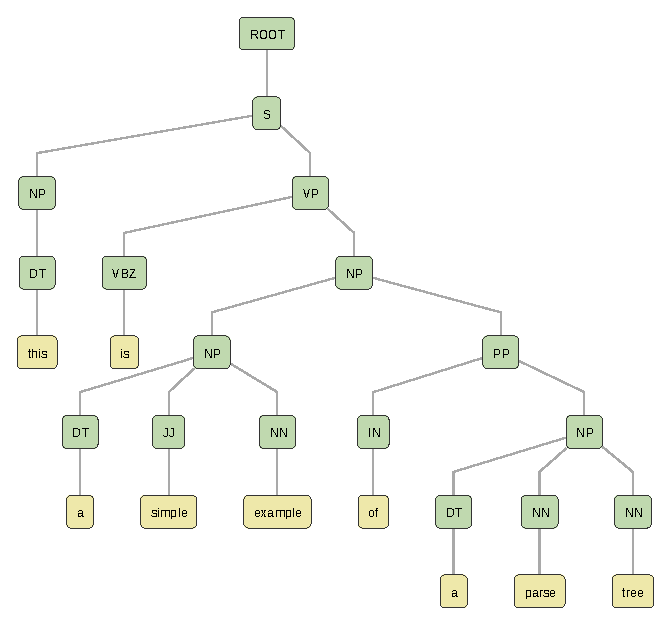
\includegraphics[width=\textwidth]{constparse}}
	\label{fig:consparse}
\end{figure}


\begin{figure}
	\caption{A dependency parse tree for the sentence \natlang{This is a simple example of a parse tree},
	This flattened view may be misleading.
	\natlang{example} is at the peak of the tree, with direct children	being:
	\natlang{this},\natlang{is},\natlang{a},\natlang{simple},
	and \natlang{tree}.
	\natlang{tree} has direct children being: \natlang{of},\natlang{a}, and \natlang{parse}.
	}
	\centering{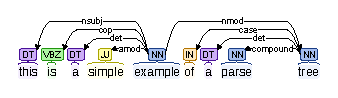
\includegraphics[width=\textwidth]{depparse}}
	\label{fig:depparse}
\end{figure}


\aside[Machine learning frameworks for structural models]{
	Structural networks can not be easily defined in most modern static neural network frameworks,	such as TensorFlow.
	These frameworks function by defining a single computational graph that is used to process each training/test case.
	The same graph is used for each input.
	By definition the structure of the network differs from training/test case to training/test case.
	Technically the same problems apply to RNNs, as each case can have a different number of inputs.
	This is normally worked around by defining the network graph for the longest input to be considered,
	then padding all the inputs to this length, and ensuring that the padding does not interfere with the gradient updates.
	The equivalent tricks for structured networks are significantly more complex.
	The exception to this is of-course via dynamic components to the static frameworks
	(which TensorFlow and other such frameworks certainly do have).
	Even in a dynamic framework it remains a non-trivial task to implement these networks.
}


\aside[Implementing Back-propagation through structure]{
	Back-propagation through structure is conceptually not significantly more complex than back propagation through time.
	However, in practice it is a very difficult algorithm to get right.
	In implementation it is very important to test for correctness using gradient checks, as it is easy to make a mistake and end-up with models that seem to work ok, but are actually crippled due to some mistake in the coding.
	Unfolding recursive autoencoders are particularly difficult,
	as the gradient must be propagated from all leaves.
	And output interior nodes can not have their gradients calculated until the gradients of their children are calculated.
	The solution to this is to process the node gradient calculation using a priority queue,
	where the priority is set by the depth of the node.
	Thus ensuring all children are processes before their parents.
}


We refer here to models incorporating tree, or graph structures as structural models.
Particular different variations have there own names, such as recursive neural networks (RvNN), and recursive autoencoders (RAE).
We use the term structural model as an all encompassing term. 
It also makes for clearer reading to distinguish recursive and recurrent  neural networks.
Just as a linked list is but a particular case of a tree, an RNN is a particular case of a structural model,
however we will exclude them from this discussion except where marked.


The initial recent work on structural models was done in for the thesis of \tcite{socher2014recursive}.
It builds on the work of \tcite{goller1996BPstructure} and \tcite{Pollack199077}, which present back-propagation through structure.
Back-propagation can be applied to networks of any structure, much like (and indeed directly because) the chain-rule can be applied to any equation, formed by the composition of differentiable functions, to find its derivative.
This means that structuring a network according to its parse structure is possible.

\subsection{Constituency Parse Tree (Binary)}
A tree structured networks function apply an recursive unit (which we will call RV) across pairs (or other groups of) the representations of the lower levels, to produce a combined representation.
A network for binary tree structured input is itself be a binary tree of RVs.
Each RV (i.e. node in the graph) can be defined by the composition function:
\begin{align}
	f_{RV}(u, v) &= \varphi\left( [S R][u;v] + b \right) \\ \label{equ:rnn1}
			     &= \varphi\left( Su +Rv + b \right)
\end{align}
where $u$ and $v$ are the left and right substructures embeddings (word embeddings at the leaf node level), and $S$ and $R$ are the matrices defining the left and right inputs are to be combined.


This is a useful form as all constituency parse trees can converted into binary parse trees, via left-factoring or right factoring (adding new nodes to the left or right to take some of the children).
This is sometimes called binarization, or putting them into  Chomsky normal form.
This is the form of structured network has been used in many words, including \tcite{socher2010PhraseEmbedding}, \textcite{SocherEtAl2011:RAE},  \textcite{SocherEtAl2011:PoolRAE},
 \textcite{Socher2011ParsingPhrases} and \textcite{zhang2014BRAE}.
Notice that $S$ and $R$ matrices are shared for all RVs, so all substructures are composed the in the same way, based only on if they are on the left, or the right.

\subsection{Dependency Tree}
In dependency tree based structured RNNS, such as in \tcite{socherDTRNN}, \tcite{iyyer2014neural}, and \tcite{iyyer2014generating},
it is possibly to the dependency relationships to switch in use different composition matrices into the RV.
This allows for multiple inputs to a single head node distinguished by their relationship rather than their order.
This is important for networks using a dependency parse tree structure, and this structure allows a node to have any number of inputs.
If we have a function $r(i,j)$ giving the relationship between head word $i$ and the word $j$, e.g. giving back \natlang{nsub}, \natlang{det}, \natlang{nmod}, \natlang{case} etc.
Then the composed representation at each RV is given by 
\begin{align}
	f_{RV}(i) &= \varphi\left(W_{head} C_{w_i} + \sum_{j \in \mathrm{children}(i)} W_{r(i,j)} \, f_{RV}(j) + b \right)
\end{align}
Here $C_{w_i}$ is the word embedding for $w_i$, and $W_{head}$ encodes the contribition of the headword to the composed representation.
Note that the terminal case is just $f_{RV}(i) = \varphi \left( W_{head} C_{w_i} + b \right)$ when a node $i$ has no children.
By using the relationship to determined the composition matrix, it increase both the networks expressiveness, and also handled the non-binary nature of dependency trees.


A similar technique could be applied to constituency part trees.
This would be using the part of speech (e.g. VBZ, NN) and phrase tags (e.g. NP, VP) for the substructures to choose the weight matrix.
This would however lose order information in some cases, where multiple inputs have the same tag.

The next step along this line of reasoning is to allow the input below to not only determine the embedding vector input but also to determine the matrices used to encode the relationship.
So not only is the representation of the (sub)prase determined by a relationship between  its constituents (as represented by there embeddings),
but the nature of that relationship (as represented by the matrix) is also determined by the constituents.
In this approach at the left-nodes every word has not only a word vector, but also a word matrix.
This is discussed in \Cref{sec:matrix-vector-models}


\pdfcomment{Maybe all these applications should be moved}
\subsection{Parsing}
The initial work for both contingency tree structured networks  \parencite{socher2010PhraseEmbedding} and for dependency tree structured networks \pcite{stenetorp2013transition} was on the creation of parsers.
This is actually rather different to the works that followed.
In that in most other work the structure is provided as part of the input.
Where-as the parser must induce the structure of the network,
from the unstructured input text.
This is simpler for the contingency parsing.

In a binary contingency parse any pair of nodes can only be merged with an adjacent node.
The process is to consider which nodes are to be composed into a higher level structure.
For each pair of adjacent nodes, an RV can be applied to get a merged representation.
A linear scoring function was also learned, that took a merged representation and determined how good it was.
This was trained such that correct merges scored highly.
This was done using hinge loss, functioning similarly to negative sampling (\Cref{sec:negative-sampling}) to cause the merged actually done in the training set to score well.
To perform the parse, nodes were merged.
Replacing them with their composed representation, and the new adjacent pairing score must be recomputed.
\textcite{socher2010PhraseEmbedding} considered both greedy, and dynamic programming search to determine the order of composition, as well as a number of variants to add additional information to the process.
The final parser performed almost as well as the state-of-the-art parser.
The dependency tree parser extends beyond this method


Dependency trees can have child-nodes that do not correspond to adjacent words (non-projective language).
This means the parser must consider that any node could have a link added to any other node (that was not already linked).
Traditional transition-based dependency parsers function by iteratively predicting links (transition) to add to the structure based on its current state.
\textcite{stenetorp2013transition}  observed that a composed representation given similarly to in \Cref{equ:rnn1}, was an ideal input to a softmax classifier that would predict the next link to make.
Conversely, the representation that is suitable for predicting the next link to make, is itself a composed representation.
Note, that \textcite{stenetorp2013transition}, unlike in future dependency tree structured RNN, uses the same matrices for all relationships; as the relationships must determined from the links made, so cannot readily be used in determining if those links are to be made.
More recent advancements in dependency tree parsing using structured networks are considered by \tcite{bowman2016fast}.




\subsection{Recursive Autoencoders}
\aside[Application to image retrieval]{An interesting application of structured networks was shown in \textcite{socherDTRNN}.
	A dependency tree structured network was trained on a language modelling task (Not as a recursive autoencoder, although that would also have been a valid option.).
	Then, separately a convolutional neural network was trained to produce a vector output of the same dimensionality -- an image embedding -- such that its distance to its caption's composed vector representation was minimised.
	The effect of this was to that images and there captions are projected to a common vector space.
	This allowed for smart image retrieval, from discriptions, by having a set of all images, and storing their embedding representations,
	then for any query, the composed embedding can be found and the vector space of images can be search for the nearest.
	(the reverse is not generally as useful, as one can't reasonably store all possible captions describing an image, so as to be able to search for the best one for an user provided image.)
	This can be done with any sequence representation.
	Further, as discussed in \Cref{sec:aligning-vector-spaces-across-languages} it can also be done post-embedding determination on both sides using (kernel) CCA.
}

Recursive autoencoders are autoencoders, just as the autoencoder discussed in \Cref{sec:bottle-necking-autoencoder} they reproduce there input.
It should be noted that unlike the encoder-decoder RNN discussed above, e.g. \Cref{sec:vae-and-encoder-decoder},
they can not be trivially used to generate natural language from an arbitrary embeddings, as they require the knowledge of the tree structured to unfold into.
Solving this would be the inverse problem of parsing to a composed representation discussed above.

The models presented in \textcite{SocherEtAl2011:PoolRAE} and \textcite{iyyer2014generating}
are unfolding recursive autoencoders ).
In these models there an identical inverse tree is defined above the highest node.
The loss function is the sum of the errors at the leaves i.e. the distance in vector space between the reconstructed words embeddings and the input word-embeddings.
This was based on a simpler earlier model.


The normal Recursive Autoencoder,
as was used in \textcite{SocherEtAl2011:RAE} and \textcite{zhang2014BRAE} only performs the unfold at each node.
That means that it assesses if each merge can be reconstructured, uses errors in the vector space to its inputs embeddings.
Those inputs are not word embedding, except when the inputs happen to both be leaf nodes.
This covers the auto-encoding nature of each merge;
but does not give any direct promise of the auto-encoding nature of the whole structure.
It should be noted that while it is not trained for, the reconstruction components (that during training are applied only at nodes) can never the less be applied recursively from the top layer, to allow full reconstruction
Though it is possible to use the learned reconstruction network components recursively from the top layer just like in the unfolding case.

\subsubsection{Semi-supervised}
In the case of all these autoencoders, except \textcite{iyyer2014generating}, a second source of information is also used to calculate the loss during training.
The networks are being simultaneously trained to perform a task.
This is often considered as semi-supervisors learning, as unlabelled data can be used to train the auto-encoding part (unsupervised) gaining good representation, and labelled data can be used train the supervised part making that representation useful for the task.
This is done by imposing an additional loss function onto the output of the central/top node.
\begin{itemize}
 \item In \textcite{SocherEtAl2011:RAE} this was for sentiment analysis.
 \item In \textcite{SocherEtAl2011:PoolRAE} this was paraphrase detection.
 \item In \textcite{zhang2014BRAE} this was the distance between embeddings of equivalent translated phrases for two RAEs for different languages.
\end{itemize}
The reconstruction loss and the supervised loss can be summed, optimised in alternating sequence, or the reconstructed loss can be optimised first, then the labelled data used for fine-tuning.

 


\aside[Sequential models are often preferred to structural models]{
Sequential (RNN) models are much more heavily researched than structural (RvNN) models.
They have better software libraries, and are easier to implement.
In theory it is possible for a sequential model (with sufficiently deep and wide RUs) internalise the connections that a structural model would posses.
While structural models are theoretically nicer from a linguistics standpoint, pragmatically they are the last resort in modelling.
When attempting to find an useful representation of a sentence for a task, one should first try a sum of word embeddings with a simple network on-top,
then sequential model (based on LSTM or GRU), and only if these fail then try a structured model.
Arguably before using any neural network approach at all, one should eliminated bag of words, bag of ngrams, dimensionality reduced version of those bags, and also eliminated LSI and LDA as inputs for the task.
Simple is powerful.
}




\section{Matrix Vector Models}\label{sec:matrix-vector-models}
\subsection{Structured Matrix Vector Model}
\aside[Dependency Tree Extension]{
	It is interesting to consider how one might extend this structure for dependency parse trees.
	We suggest the logical change would be for the $R$ and $S$ matrices to be determined by the relationship of the child node (including \emph{head}),
	Or the $W$ matrix to be determined by the relationship of the head to its own parent (potentially the fake relationship \emph{root}).
	To do both seems redundant (though perhaps no more so than having $W$ in the first place).
	Similar, based on POS could be done for the constituency parse tree.
}

\tcite{SocherMVRNN} proposed that each node in the graph should define not only a vector embedding, but a matrix defining how it was to be combined with other nodes.
That is to say, each word and each phrase has both an embedding, and a composition matrix.

This considered this for binary constituency parse trees.
The composition function is as follows:
\begin{align}
f_{RV}(u, v, U, V) &= \varphi\left( [S;R][Uv;Vu] + b \right) \\ 
&= \varphi\left( SUv +RVu + b \right)\\
F_{RV}(U, V) = W[U;V] = W_L U + W_R V
\end{align}


$f_{RV}$ gives the composed embedding, and $F_{RV}$ gives the composing matrix.
$S$ and $R$ represent the left and right composition matrix components that are the same for all nodes (regardless of content).
$U$ and $V$ represent the per word/node child composition matrix components.
(We note that $S$ and $R$ could in theory be rolled in to $U$ and $R$ as part of the learning)
$u$ and $v$ represent the per word/node children embeddings.
$W$ represents the method for merging two composition matrices.

We note that one can define increasingly complex and powerful structured networks along these lines; though one does run the risk of over-fitting, and very long training times.

\subsection{Sequential Matrix Vector Model}
\pdfcomment{Maybe this section should just move to the RNN section/chapter}
A similar approach, of capturing a per word matrix, 
was used on a sequential model by \tcite{rui2017mvrusemantic}.
While sequential models are a special case of structured models,
it should be noted that unlike the structured models discussed prior,
this matrix vector RNN features gated memory.
This matrix-vector RNN is an extension of the GRU discussed in \Cref{sec:rnn}, but without a reset gate.


In this sequential model, advancing a time step, is to perform a composition.
This composition is for between the input word and the (previous) state.
Rather than directly between two nodes in the network as in the structural case.
It should be understood that composing with the the state is not the same as composing the current input with the previous input.
But rather as composing the current input with all previous inputs (though not equally).

In this method each word, $w_t$ is represented by a word embedding $x_{w_t}$ and matrix: $X_{w_t}$, these are the inputs at each time step.
The network outputs and states are the composed embedding $\hat{y}_t$ and matrix $Y_t$.

\pdfcomment{Subscripts in this section mean time, not index.}

\aside[Remember:]{The product of a matrix with a concatenated vector, is the same as the sum of the two blocks of that matrix each multiplied by the blocks of that vector.}
 
\begin{align}
h_t &= \tanh\left(V[x_t; \hat{y}_{t-1}] + c \right)\\
z_t &= \sigma\left(Y_{t-1}x_t + X_t \hat{y}_{t-1} + k \right)\\
%
\hat{y}_t &= r_t \odot c_t + (1-r_t) \odot \hat{y}_{t-1} \\
Y_t &= \tanh \left( W[Y_{t-1}; X_t] + b \right)
\end{align}



The matrices $W$ and $V$ are shared across all time steps/compositions.
$U$ controls how the next state-composition $Y_t$ matrix is generated from its previous value and the input composition matrix: $X_t$.
$V$ similarly controls the value of the candidate state-embedding $h_t$.

$h_t$ is the candidate composed embedding (to be output/used as state).
$z_t$ is the update gate, it controls how much of the actual composed embedding ($\hat{y}_t$) comes from the candidate $h_t$ and how much comes from the previous value ($\hat{y}_{t-1}$).
The composition matrix $Y_t$ (which is also part of the state/output) is not gated.

Notice, that the state composition matrix $Y_{t-1}$ is only used to control the gate $z_t$, not to directly effect the candidate composited embedding $h_t$.
Indeed, in fact one can note that all similarity to the structural method of \textcite{SocherMVRNN} is applied in the gate $r_t$.
$h_t$ is similar to in a normal RU.



\begin{figure}
	\caption{A Matrix Vector Recurrent unit, that an RNN could be made from}
	\label{fig:mvrnn}
	\begin{adjustbox}{max width=\textwidth}
		\begin{tikzpicture}[]
		\node(hidden)[layer]{$h_t = \tanh\left(V[x_t; \hat{y}_{t-1}] + c \right)$};
		\node(update)[layer, left=of hidden]{$z_t = \sigma\left(Y_{t-1}x_t + X_t \hat{y}_{t-1} + k \right)$};
		\node(state)[layer, above = 4 of update]{$\hat{y}_t = r_t \odot c_t + (1-r_t) \odot \hat{y}_{t-1}$};
		
		\node(matrix)[layer, above left = of update]{$Y_t = \tanh \left( U[Y_{t-1}; X_t] + b \right)$};
		
		\draw[->] (update) edge node[labe] {$z_{t}$} (state.south);		
		\draw[->] (hidden) edge node[labe] {$h_{t}$} (state.south);
		
		
		
		\node(in)[below = 4 of update]{input};
		\node(inX)[above = 0 of in.north west]{$X_t$};
		\node(inx)[above = 0 of in.north east]{$x_t$};
		
		\draw[->] (inX) edge node[labe] {$X_t$} (matrix);
		\draw[->] (inx) edge node[labe] {$x_t$} (hidden);
		\draw[->] (inx) edge node[labe] {$x_t$} (update);
		
		\node(stm)[left = 9 of update]{old state};
		\node(stmY)[below = 0 of stm.south east]{$Y_{t-1}$};
		\node(stmy)[below = 0 of stm.south west]{$\hat{y}_{t-1}$};
		
		
		\draw[->, bend right] (stmy) edge node[labe] {$\hat{y}_{t-1}$} (update.south);
		\draw[->, bend right] (stmy) edge node[labe] {$\hat{y}_{t-1}$} (hidden.south);
		\draw[->, bend right] (stmy) edge node[labe] {$y_{t-1}$} (state.south);
		
		\draw[->, bend right] (stmY) edge node[labe] {$Y_{t-1}$} (update.south);
		\draw[->, bend right] (stmY) edge node[labe] {$Y_{t-1}$} (matrix.south);
				
		
		\node(stp)[above = 2 of state.west]{new state\\i.e output};
		\node(stpY)[below = 0 of stp.south west]{$Y_{t}$};
		\node(stpy)[below = 0 of stp.south east]{$\hat{y}_{t}$};

		\draw[->] (matrix) edge node[labe] {$Y_{t}$} (stpY);
		\draw[->] (state) edge node[labe] {$\hat{y}_t$} (stpy);

		
		\node(updatelbl)[labe, above= 0 of update]{Update Gate};
		\node(hiddenlbl)[labe, above= 0 of hidden]{Candidate New State Vector};
		\node(matrixlbl)[labe, above= 0 of matrix]{New State Matrix};
		\end{tikzpicture}
	\end{adjustbox}
\end{figure}

\pdfcomment{Say somehting about targeting short phrases and the missing gates?}



\section{Implementations}

The implementation of \tcite{socher2010PhraseEmbedding}, is publicly available,
however it does not export embeddings.
It is nested deep in side the Stanford Parser (Java), accessing the embeddings is highly non-trivial.

There is a popular implementation the paragraph vector models in recent versions of the python gensim library \pcite{rehurek_lrec}, along with many information retrieval vector models such as LDA.


\section{Conclusion}

\subsection{On compositionality}
\tcite{Mitchell2008} \pdfcomment{Incorperate this}

It is tempting to think of the structured models as compositional,
and the sequential models as non-compositional.
However, this is incorrect.

The compositional nature of the structured models is obvious:
the vector a phrase is composed from the vectors of the words the phrase are formed from.

Sequential model are able to learn learning the structures.
For example, learning that a word from X time steps ago is to be remembered in the RNN state, a to be meaningfully combined with the current word, in the determining of the next state.
This demonstrates the same compositionality.
It has been shown that sequential models are indeed in-practice able to learning such relationships between words \pcite{2017arXiv170909360W}.
More generally as almost all aspects of language have some degree of compositionality, and sequential models work very well on most language tasks, this implicitly shows they have sufficient representational capacity to learn sufficient degrees of compositional tasks.


\pdfcomment{I may be over highlighting this it was only 500 datums}
In fact, it has been suggested that even some unordered models such as sum of word embeddings are able to capture what would be thought of as compositional information.
This was shown by \textcite{RitterPosition}, by their ability of a na\"ive Bayes classifier with these unordered phrase representations were able predict meaning categories relationships that should only be able to be determined using a compositional understanding.
Several  sum of word embeddings no only exceeded the baseline prediction, but even out performed the structured representation from a RAE.
This suggests that a surprising amount of compositional information is being captured into the embeddings in such indexes that allows it to be represented through the addition.

We will also note that a limitation of the structural models compared to the sequential RNNs,
is there lack of explicit gating on memory (e.g. as in GRU and LSTM).
Any given path down a tree can be looked at as like an RNN comprised only of basic recurrent units.
However, these paths are much shorter (being the logarithm of) than the full sequential length of the sentence,
which offsets the need for such gating.
Recall that the gating is to provide longer short term memory.




\end{document}